\begin{center}
	\section*{Anexo A: Software de dise\~no autom\'atico}
\end{center}

\noindent
\justify

Como complemento de la metodolog\'ia de dise\~no, se desarroll\'o un software de dise\~no autom\'atico (secci\'on \ref{software}) que, adicional al desarrollo de la metodolog\'ia de c\'alculo del dise\~no anal\'itico, incorpora un m\'odulo de discretizaci\'on de dominio (pudiendo desarrollar mallas estructuras y no estructuradas) y simulaci\'on autom\'atica a trav\'es de los m\'etodos CFD y CFD-DEM. A continuaci\'on, se puede apreciar la evidencia fotogr\'afica de los componentes del software desarrollado en Python - Jupyter.

\begin{figure}[h!]
	\centering
	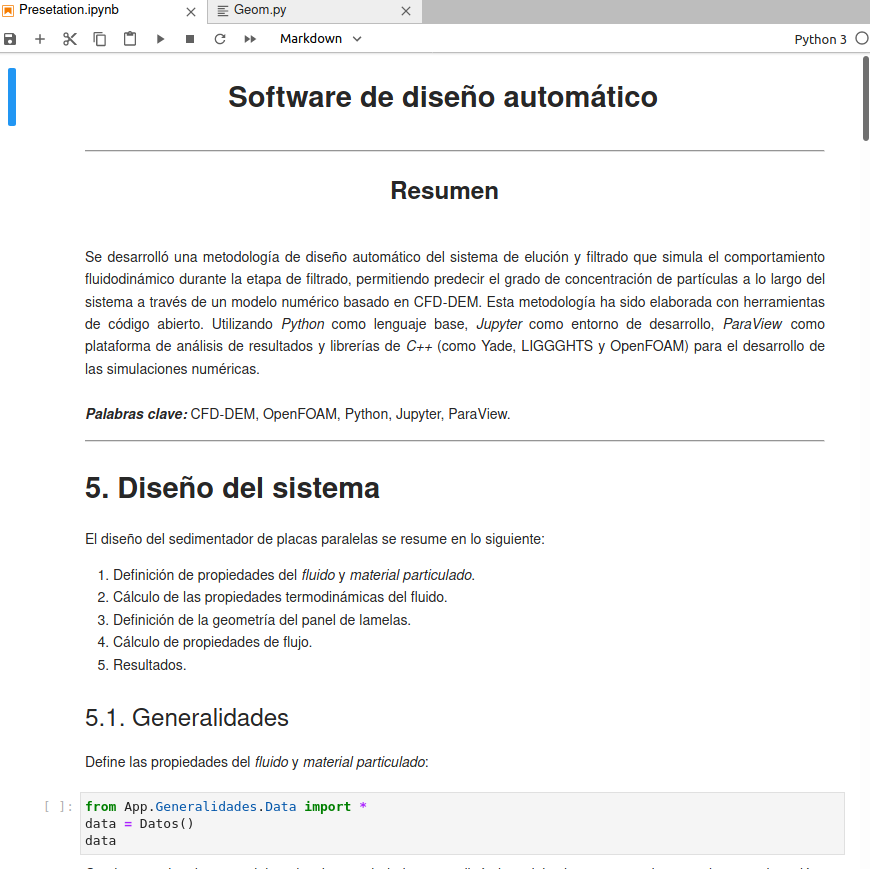
\includegraphics[width=\textwidth]{Images/Anexos/1.png}
	\caption{Inicio del software.}
	\label{inicioSoft}
\end{figure}

\noindent
\justify

Como se puede observar en la Figura \ref{inicioSoft}, el software se presenta en un formato de texto tipo pdf. Es como una especie de art\'iculo interactivo que permite ejecutar c\'odigo en vivo. El primer m\'odulo consiste en definir las condiciones de dise\~no de entrada; en t\'erminos de los datos del fluido y del material particulado. Una vez definidos los datos, se procede a calcular las propiedades termodin\'amicas.

\begin{figure}[h!]
	\centering
	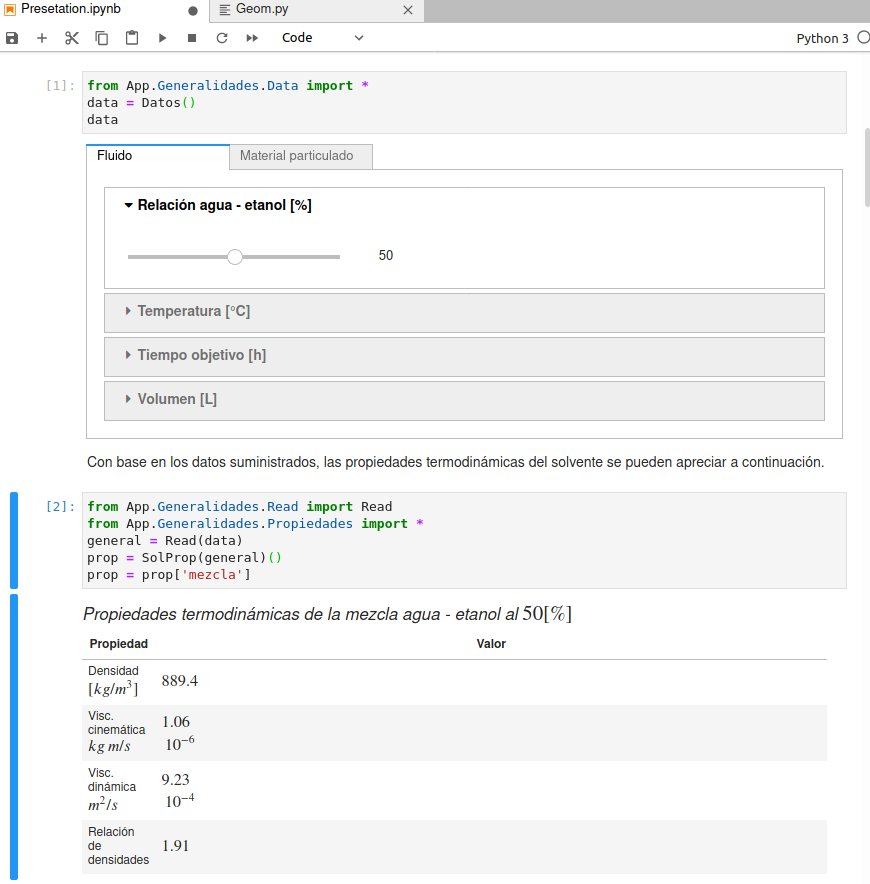
\includegraphics[width=\textwidth]{Images/Anexos/3.png}
	\caption{Datos y propiedades del solvente.}
	\label{propSoft}
\end{figure}

\newpage

\noindent
\justify

Una vez conocidas las propiedades del solvente, se procede a calcular la velocidad de asentamiento m\'axima de las part\'iculas.

\begin{figure}[h!]
	\centering
	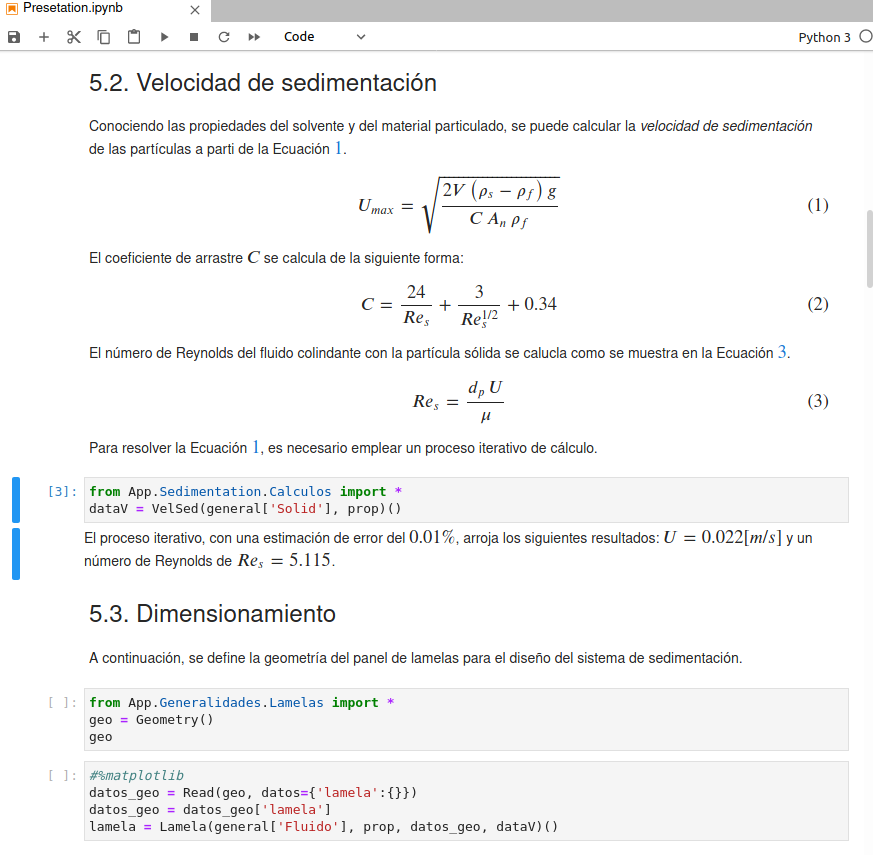
\includegraphics[width=\textwidth]{Images/Anexos/4.png}
	\caption{Velocidad de asentamiento m\'axima.}
	\label{velasSoft}
\end{figure}

\newpage

\noindent
\justify

Luego, se define una geometr\'ia inicial de dise\~no para el c\'alculo de las propiedades del fluido.

\begin{figure}[h!]
	\centering
	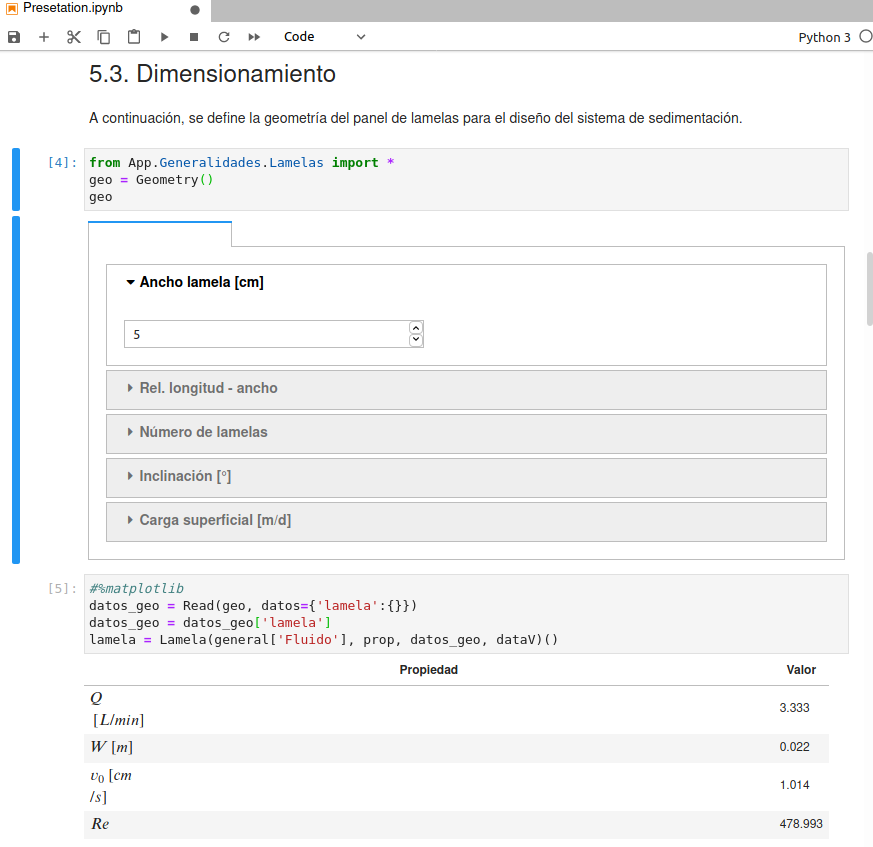
\includegraphics[width=\textwidth]{Images/Anexos/5.png}
	\caption{Geometr\'ia inicial.}
	\label{geoSoft}
\end{figure}

\newpage

\noindent
\justify

Una vez definida la geometr\'ia de estudio, con base en los criterios de dise\~no, se procede a discretizar el dominio especificando los datos referentes al mallado y al desarrollo de la geometr\'ia.

 \begin{figure}[h!]
	\centering
	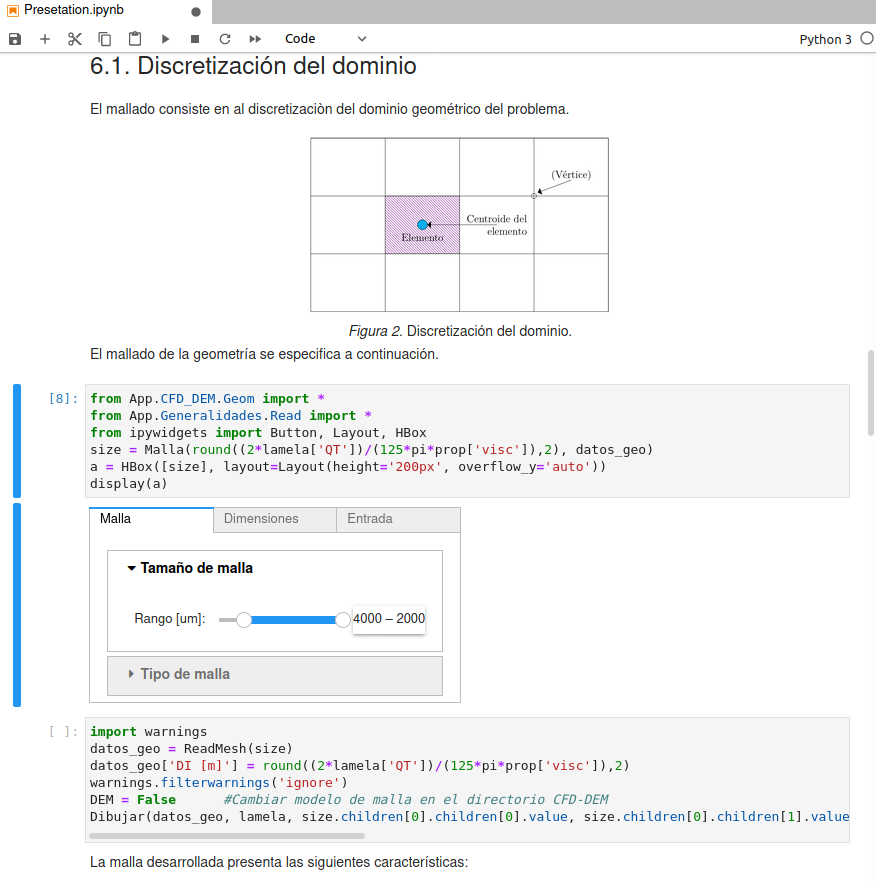
\includegraphics[width=\textwidth]{Images/Anexos/7.png}
	\caption{Datos del mallado de la geometr\'ia.}
	\label{dataMalla}
\end{figure}

\newpage

\noindent
\justify

Despu\'es, se procede a desarrollar la malla:

\begin{figure}[h!]
	\centering
	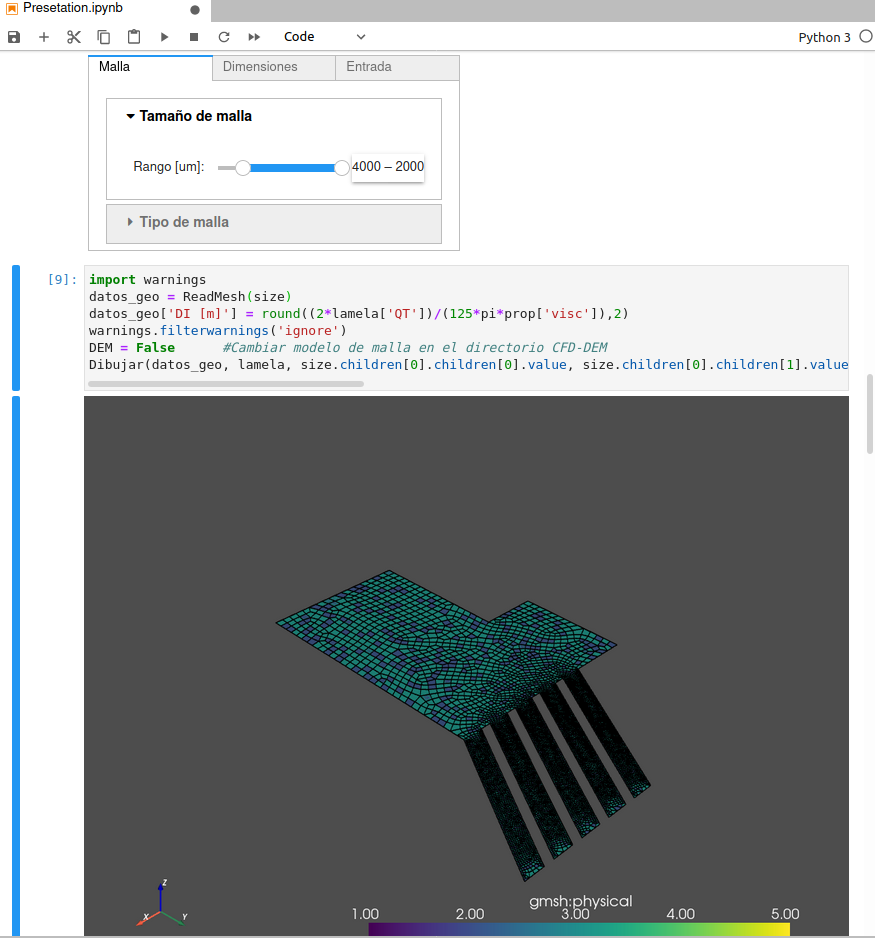
\includegraphics[width=\textwidth]{Images/Anexos/8.png}
	\caption{Mallado de la geometr\'ia.}
	\label{MallaSoft}
\end{figure}

\newpage

\noindent
\justify

Luego, se analizan las caracter\'isticas del mallado.

\begin{figure}[h!]
	\centering
	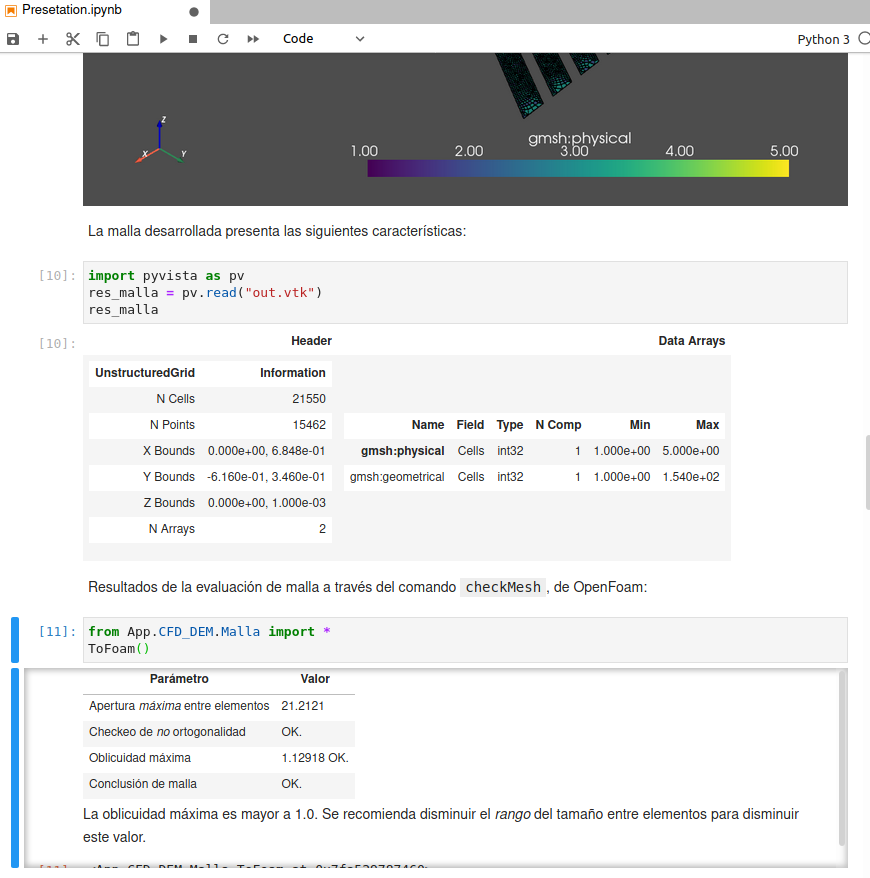
\includegraphics[width=\textwidth]{Images/Anexos/9.png}
	\caption{Caracter\'isticas del mallado.}
	\label{CarMallaSoft}
\end{figure}

\newpage

\noindent
\justify

En caso de que el mallado no sea el adecuado, es posible desarrollar cambios en los datos referentes a la geometr\'ia o al rango de tama\~nos de la malla.

\begin{figure}[h!]
	\centering
	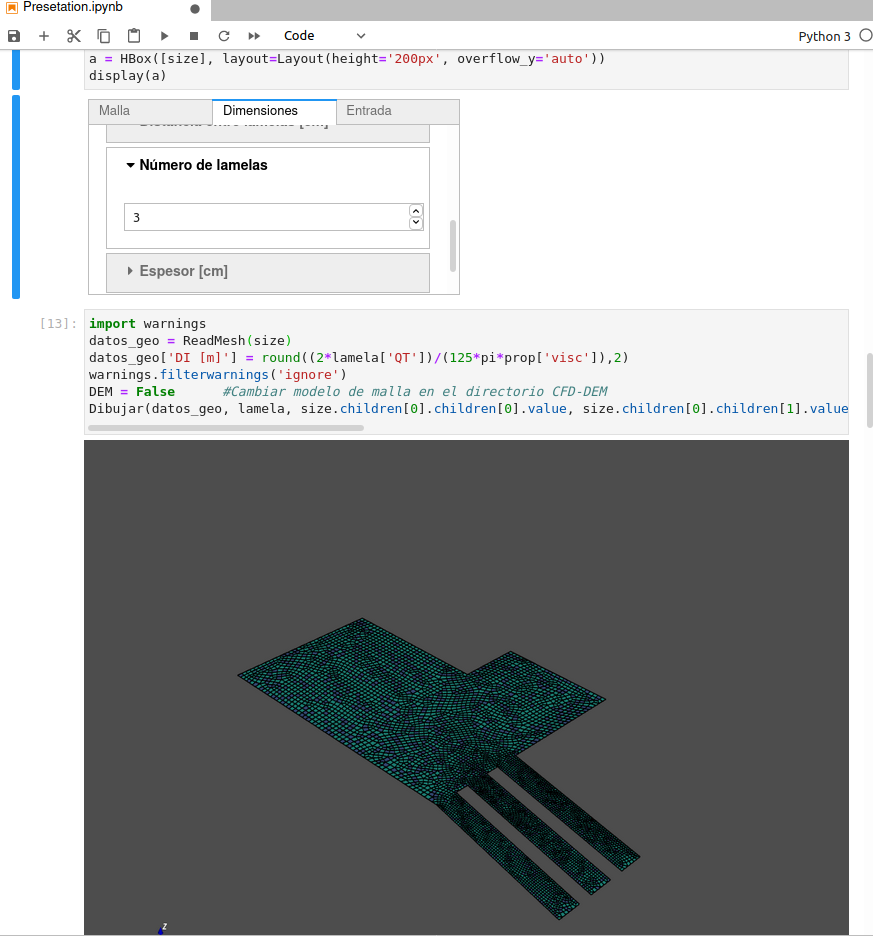
\includegraphics[width=\textwidth]{Images/Anexos/10.png}
	\caption{Cambios en el mallado.}
	\label{CamMallaSoft}
\end{figure}

\newpage

\noindent
\justify

Luego, se definen las condiciones de frontera:

\begin{figure}[h!]
	\centering
	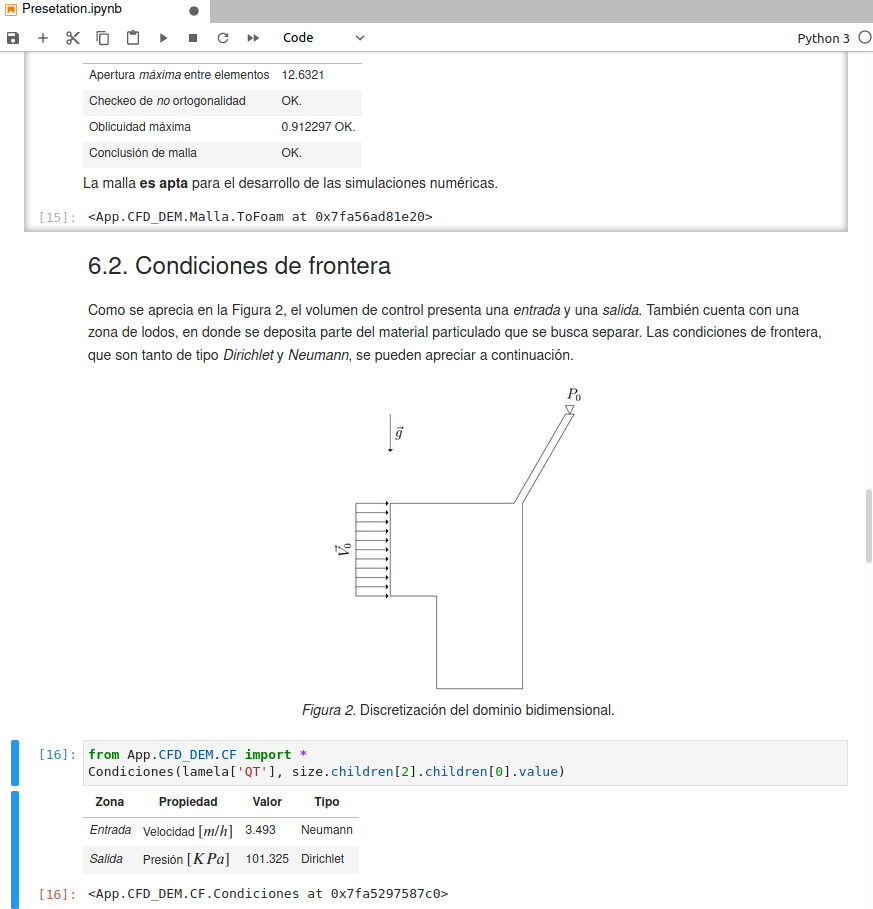
\includegraphics[width=\textwidth]{Images/Anexos/11.png}
	\caption{Cambios en el mallado.}
	\label{CamMallaSoft}
\end{figure}

\newpage

\noindent
\justify

Finalmente, se procede a realizar las simulaciones num\'ericas CFD y CFD-DEM.

\begin{figure}[h!]
	\centering
	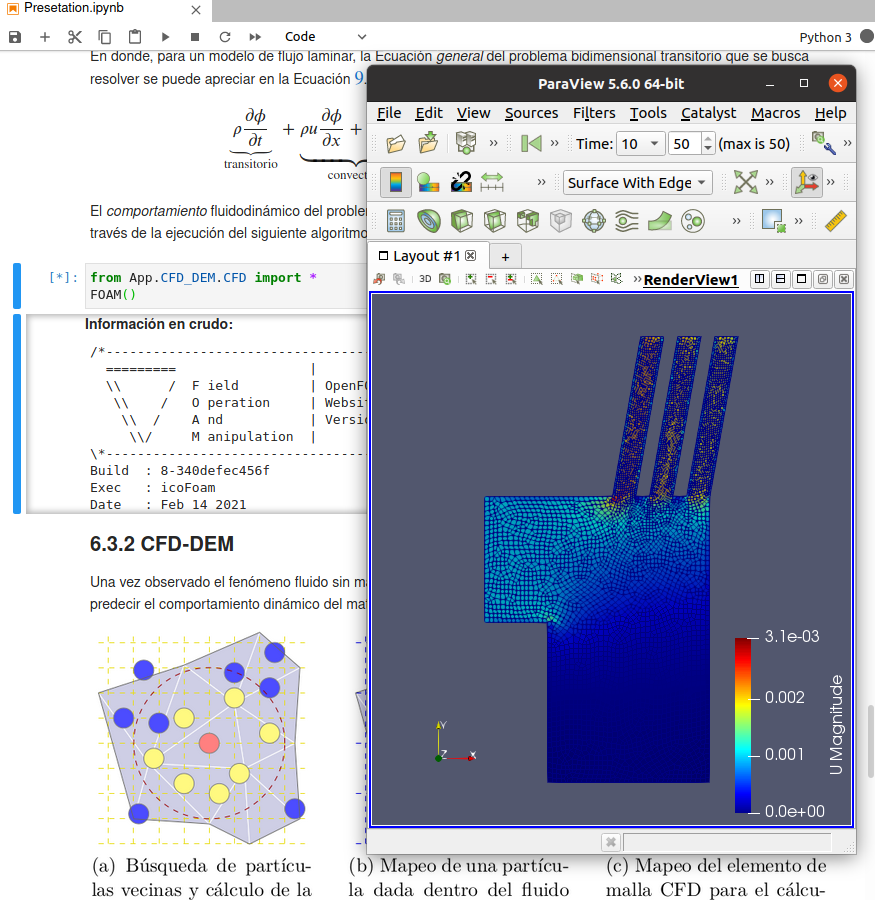
\includegraphics[width=\textwidth]{Images/Anexos/12.png}
	\caption{Cambios en el mallado.}
	\label{CamMallaSoft}
\end{figure}